\chapter{Estimation of still water depth}
%
\section{Introduction}
\par
The first image capture in an LIF sequence is of unique significance: at this stage, the camera calibration is completed, and the water surface is completely still.
With this information, the water depth can be estimated.
%
\section{The 3D problem}
\begin{figure}[H]
	\centering
	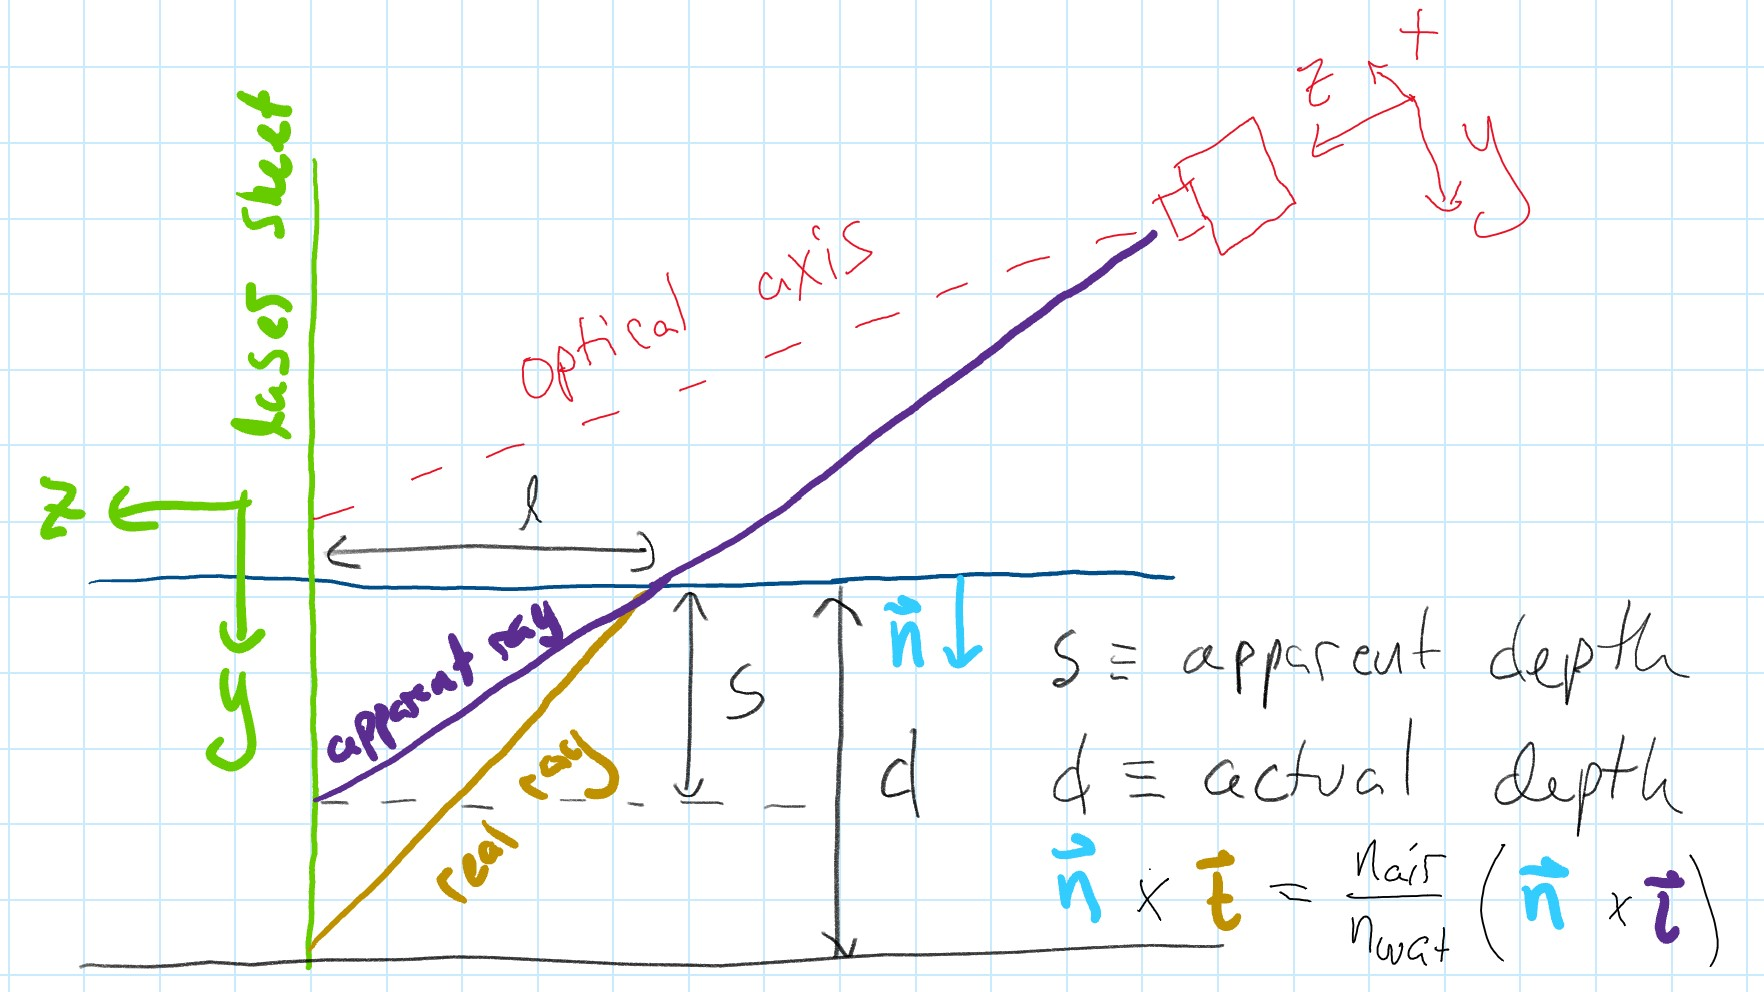
\includegraphics[width=0.75 \linewidth]{../images/depth-sketch.jpg}
	\caption{Definition sketch. Vectors in the optical coordinate, shown in red, are labeled $\vec{u}$, vectors in the laser sheet coordinate, shown in green, are labeled $\vec{X}$, the purple ray is labeled $\vec{i}$, the brown ray is labeled $\vec{t}$, the apparent depth is labeled $s$, the actual depth is labeled $d$, the normal vector to the water surface is labeled $\vec{n}$, the refractive index of air is labeled $n_{air}$, and the refractive index of water is labeled $n_{wat}$.}
	\label{fig:depth_example}
\end{figure}
\par
In three dimensions, it is easier for this problem to use linear algebra notation.
Using the calibration board, it is possible to find the change of basis $\boldsymbol{R}$ where
\begin{gather*}
	\vec{x} = \boldsymbol{R}^T \vec{u}
\end{gather*}
where $\vec{u}$ is a pixel coordinate and $\vec{x}$ is the physical coordinate system from the calibration board.
Note: here $\vec{u}$ and $\vec{x}$ are unit vectors, and so rotations are achieved, but not scaling.
Using the image of the still water surface, it is possible to find the change of basis $\boldsymbol{R'}$ where
\begin{gather*}
	\vec{X} = \boldsymbol{R'}^T \vec{x}
\end{gather*}
where $\vec{X}$ is the physical coordinate system with $X$ at the intersection of the still water surface and laser plane, $Y$ is approximately inward normal to the water surface, and $Z$ is approximately normal to the laser plane.
Again, $\vec{X}$ is a unit vector.
\par
Change of basis transformations which are pure rotations have the identity $R^{-1} = R^T$ and so
\begin{gather*}
	\vec{X} = \boldsymbol{R'}^T \boldsymbol{R}^T \vec{u}
\end{gather*}
i.e. $\vec{X}$ represents $\vec{u}$ in the laser plane coordinate.
Choosing  $\vec{u}_{bot}$ to be the pixel position of a light ray which identifies the glass bottom, the unit vector, $\vec{i}$, which represents the angle at which the light ray contacts the still water surface can be found:
\begin{gather*}
	\vec{i} = \boldsymbol{R'}^T \boldsymbol{R}^T \vec{u}_{bot}
\end{gather*}
using snells law in vector form, the unit vector $\vec{t}$ which propagates in the water can be found:
\begin{gather*}
	\vec{t} = \sqrt{\left( 1 + \left( \frac{n_{air}}{n_{wat}} \right)^2 \left[ 1 - \left(  \vec{n} \cdot \vec{i} \right)^2 \right] \right)} \vec{n} + \frac{n_{air}}{n_{wat}} \left[ \vec{i} - \left( \vec{n} \cdot \vec{i} \right) \vec{n} \right]
\end{gather*}
By scaling the vector $\vec{t}$ to have a depth of $d$, and scaling the vector $\vec{i}$ to have a depth of $s$, they both must traverse the same lateral distance, $l$.
This establishes the relationship:
\begin{gather*}
	\frac{d}{s} = \frac{i_3 t_2}{i_2 t_3}
\end{gather*}
where $i_2$ and $t_2$ are the components of the vectors which point downward, $i_3$ and $t_3$ are the components of the vectors which point normal to the laser plane.
\par
Lastly, note that the apparent water depth $s$ and consequently $d$ can be found:
\begin{gather*}
	s = \left( \boldsymbol{H} \vec{u}_{top} - \boldsymbol{H} \vec{u}_{bot} \right) \cdot \vec{n} \\
	d =\frac{i_3 t_2}{i_2 t_3}  \left( \boldsymbol{H} \vec{u}_{top} - \boldsymbol{H} \vec{u}_{bot} \right) \cdot \vec{n}
\end{gather*}
where $\vec{u}_{top}$ is the pixel position of the water surface, and $\vec{u}_{bot}$ is the pixel position of the glass bottom as identified in the image, and $\boldsymbol{H}$ is found in the typical way.
Now, the water depth $d$ can be calculated with the lens intrinsic parameters, a photo of a calibration grid, and a LIF photo of the still water condition.
%
\section{Example}
\par
Consider the following calibration image and still water image:
\begin{figure}[H]
	\centering
	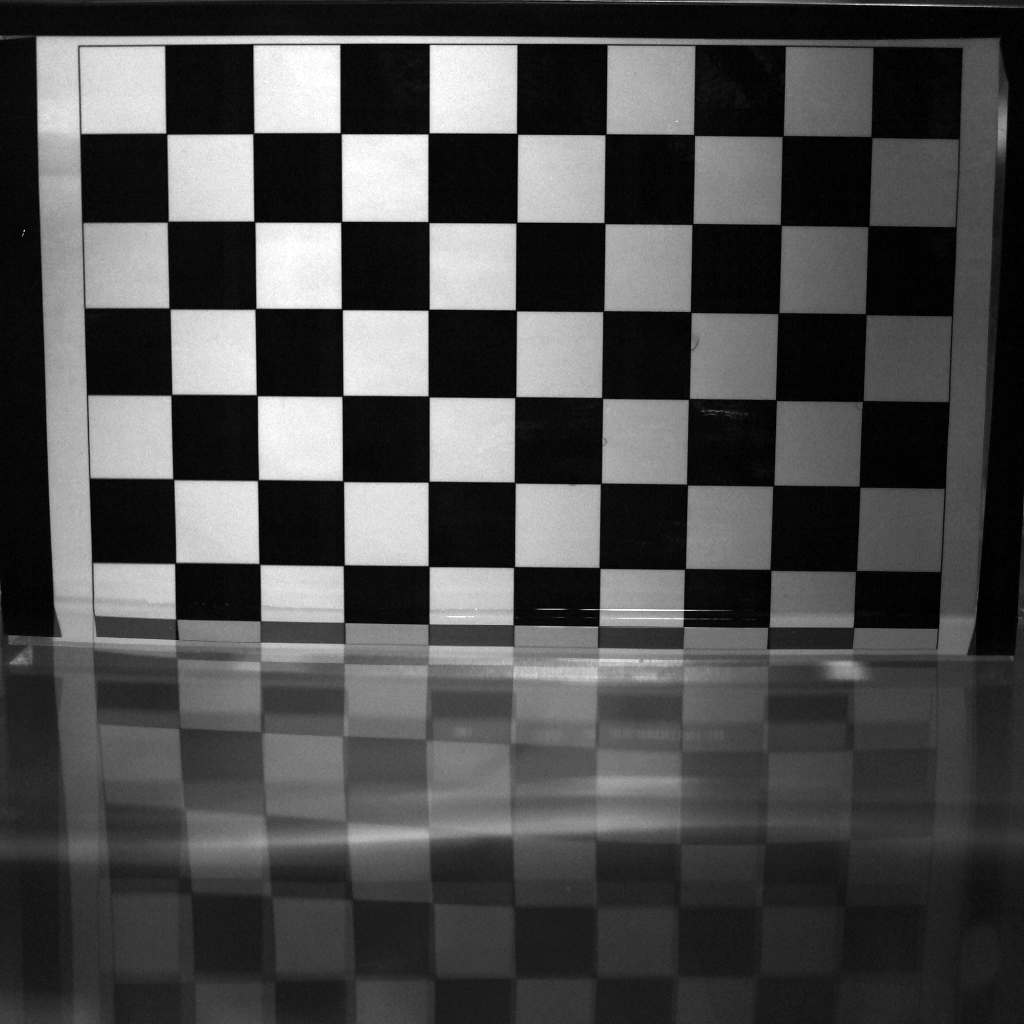
\includegraphics[width=0.45 \linewidth]{../images/depth-example-calib.png}
	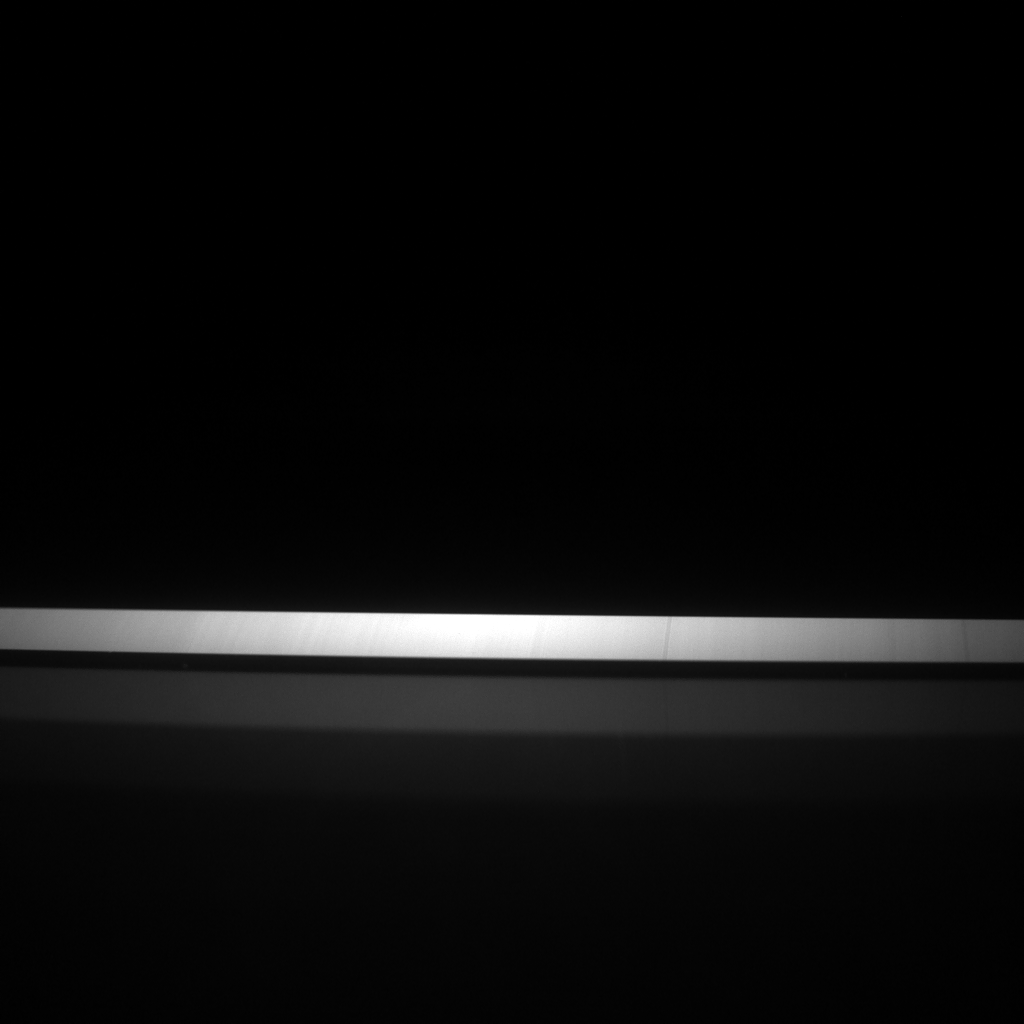
\includegraphics[width=0.45 \linewidth]{../images/depth-example-LIF.png}
	\caption{Example still water condition.
		Calibration board shown left, still water surface shown right.}
	\label{fig:depth_example}
\end{figure}
the intrinsic camera matrix is given:
\begin{gather*}
	\boldsymbol{A} =
	\begin{bmatrix}
	f_x & 0 & c_x \\
	0 & f_y & c_y \\
	0 & 0 & 1 \\
	\end{bmatrix}
	=
	\begin{bmatrix}
	1895.89 & 0 & 503.09 \\
	0 & 1895.78 & 524.40 \\
	0 & 0 & 1 \\
	\end{bmatrix}
	\text{\quad ; \quad}
\end{gather*}
the rotation matrix from pixel coordinates to calibration grid coordinates is calculated 
\begin{gather*}
	\boldsymbol{R}^T =
	\begin{bmatrix}
	0.99947801 & -0.00392189 & -0.03206767 \\
	0.00959514 & 0.98385068 & 0.17873383 \\
	0.03084882 & -0.17894823 & 0.98337474 \\
	\end{bmatrix} \text{\quad ; \quad}
\end{gather*}
and the rotation matrix from calibration grid coordinates to world coordinates is calculated
\begin{gather*}
	\boldsymbol{R'}^T = 
	\begin{bmatrix}
	0.999928 & 0.01199971 & 0. \\
	-0.01199971 & 0.999928 & 0. \\
	0. & 0. & 1. \\
	\end{bmatrix} \text{\quad ; \quad}
\end{gather*}
the apparent depth is calculated for all pixel positions is calculated
\begin{figure}[H]
	\centering
	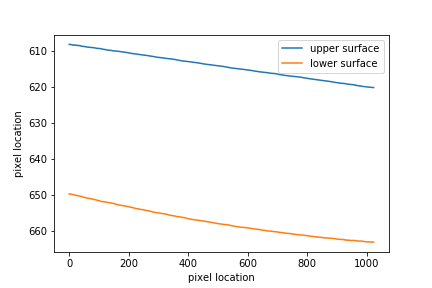
\includegraphics[width=0.45 \linewidth]{../images/depth-example-pixel-locs.png}
	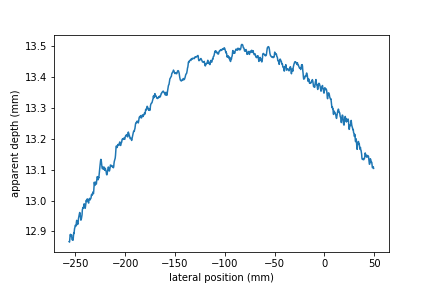
\includegraphics[width=0.45 \linewidth]{../images/depth-example-apparent.png}
	\caption{Apparent depth from example.
		Pixel location of upper and lower surface shown left, apparent water depth shown right.}
	\label{fig:depth_example_apparent}
\end{figure}
lastly, the actual water depth can be estimated
\begin{figure}[H]
	\centering
	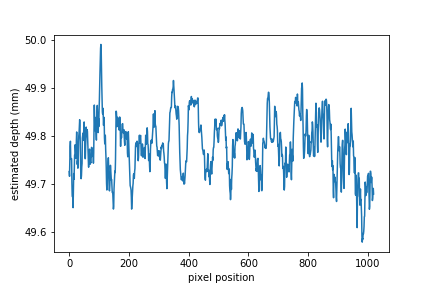
\includegraphics[width=0.45 \linewidth]{../images/depth-example-estimated.png}
	\caption{Estimated water depth from example.}
	\label{fig:depth_example_estimated}
\end{figure}
